\documentclass{beamer}
\setbeamertemplate{caption}[numbered]

\usetheme{Madrid}

% locale settings 
\usepackage[T2A]{fontenc}
\usepackage[utf8]{inputenc}
\usepackage[english,russian]{babel}

% graphics settings
\usepackage[compatibility=false]{caption}
\usepackage{subcaption}
\usepackage{wrapfig}
\usepackage{graphics, graphicx}
\graphicspath{{./images/}}

% hyperlinks settings
\usepackage{hyperref}
\hypersetup{unicode=true}

\title{Анализ данных кинопоиска}
\author{Курносов Дмитрий, Лансков Никита, Нахатович Михаил, Смольский Максим }
\date{18 декабря, 2020}
\subtitle{3640102/00201}

\begin{document}
	\frame {
		\titlepage
	}
	\frame {
		\frametitle{Кратко о кинопоиске}
		
		КиноПоиск - крупнейший русскоязычный интернет-сервис о кино. Содержит
		информацию о различных фильмах, которой мы воспользовались для решения 
		поставленных статистических и исследовательских задач.
	}
	\frame {
		\frametitle{Архитектура проекта}
		\begin{figure}
			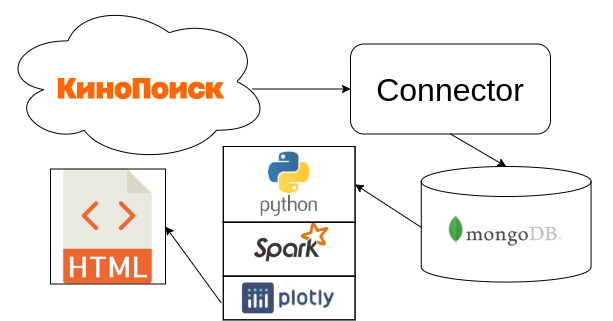
\includegraphics[width=\linewidth]{architecture}
			\label{fig:1}
		\end{figure}
	}
	\frame {
		\frametitle{Получение данных}
	}	
	\frame {
		\frametitle{Структура данных}
	}
	\frame {
		\frametitle{Статистические задачи}

		\begin{itemize}
			\item Корелляция оценок зрителей и критиков
			\item Распределение фильмов по странам
			\item Распределение фильмов по прибыльности			
			\item Распределение фильмов по странам и годам
			\item Распределение фильмов по возрастным ограничениям и годам
			\item Средний рейтинг российских фильмов по годам			
		\end{itemize}
	}
	\frame {
		\frametitle{Корелляция оценок зрителей и критиков}
	}
	\frame {
		\frametitle{Распределение фильмов по странам}
	}
	\frame {
		\frametitle{Распределение фильмов по прибыльности (1)}
		\begin{figure}
			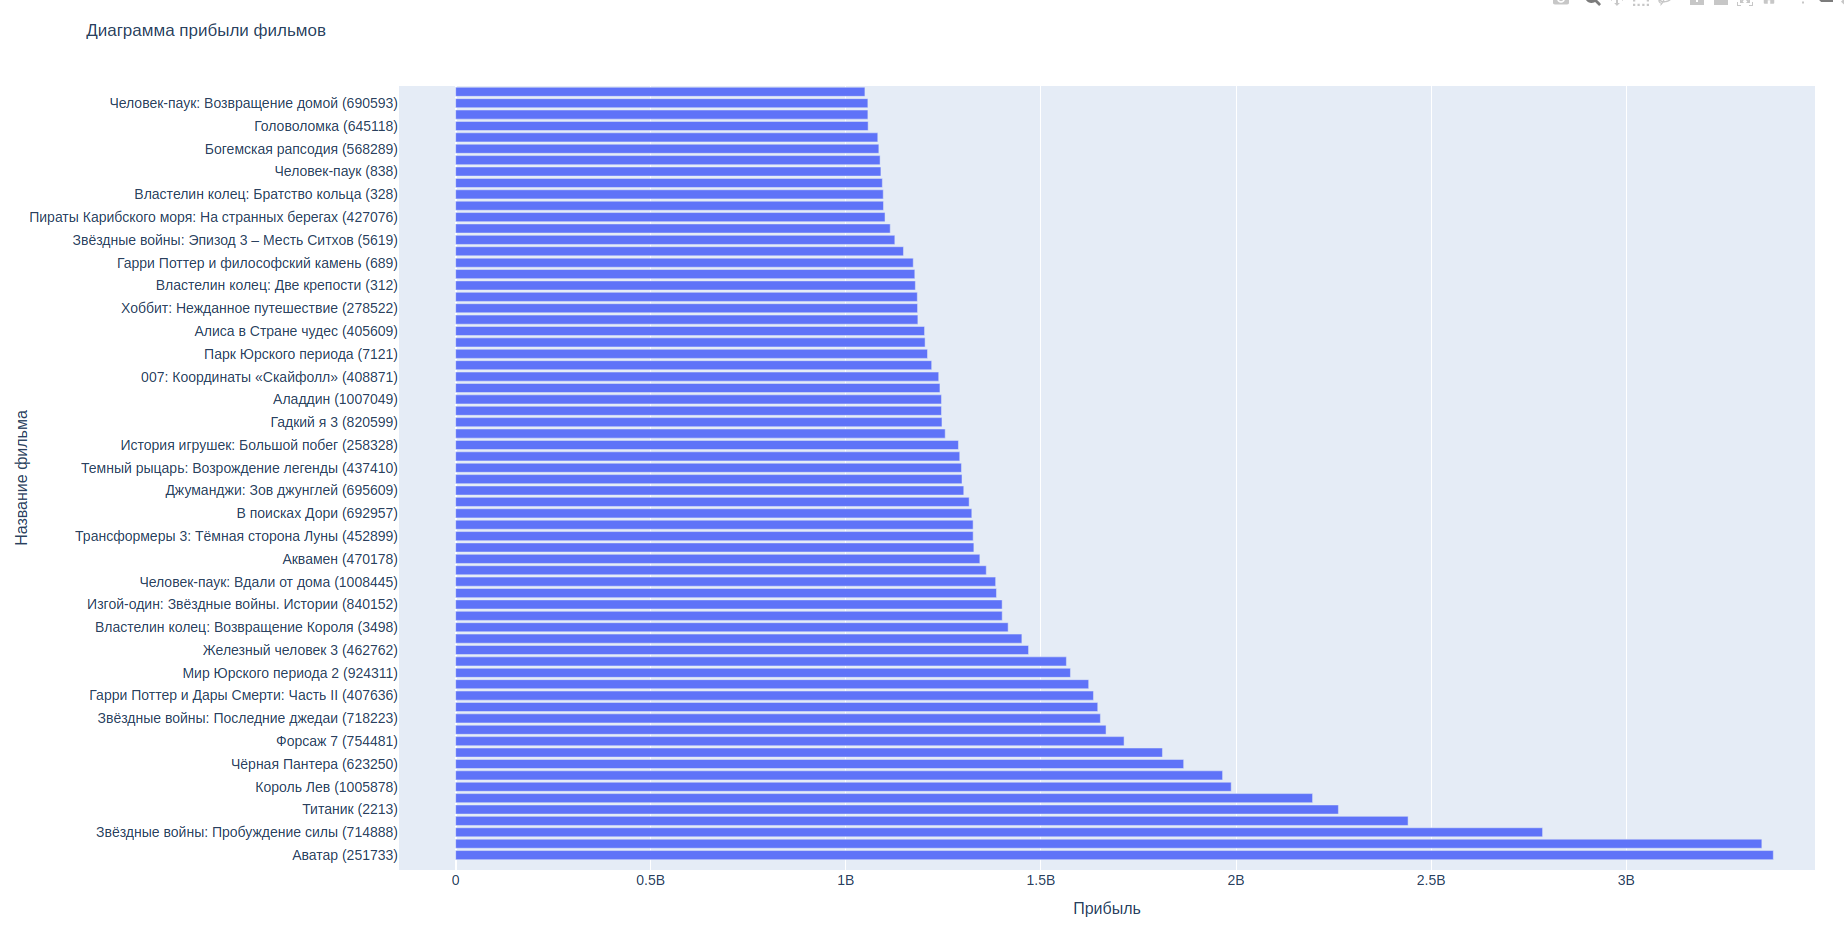
\includegraphics[width=\linewidth]{profit/best}
			\caption{Самые прибыльные фильмы}
			\label{fig:2}
		\end{figure}
	}
	\frame {
		\frametitle{Распределение фильмов по прибыльности (2)}
		\begin{figure}
			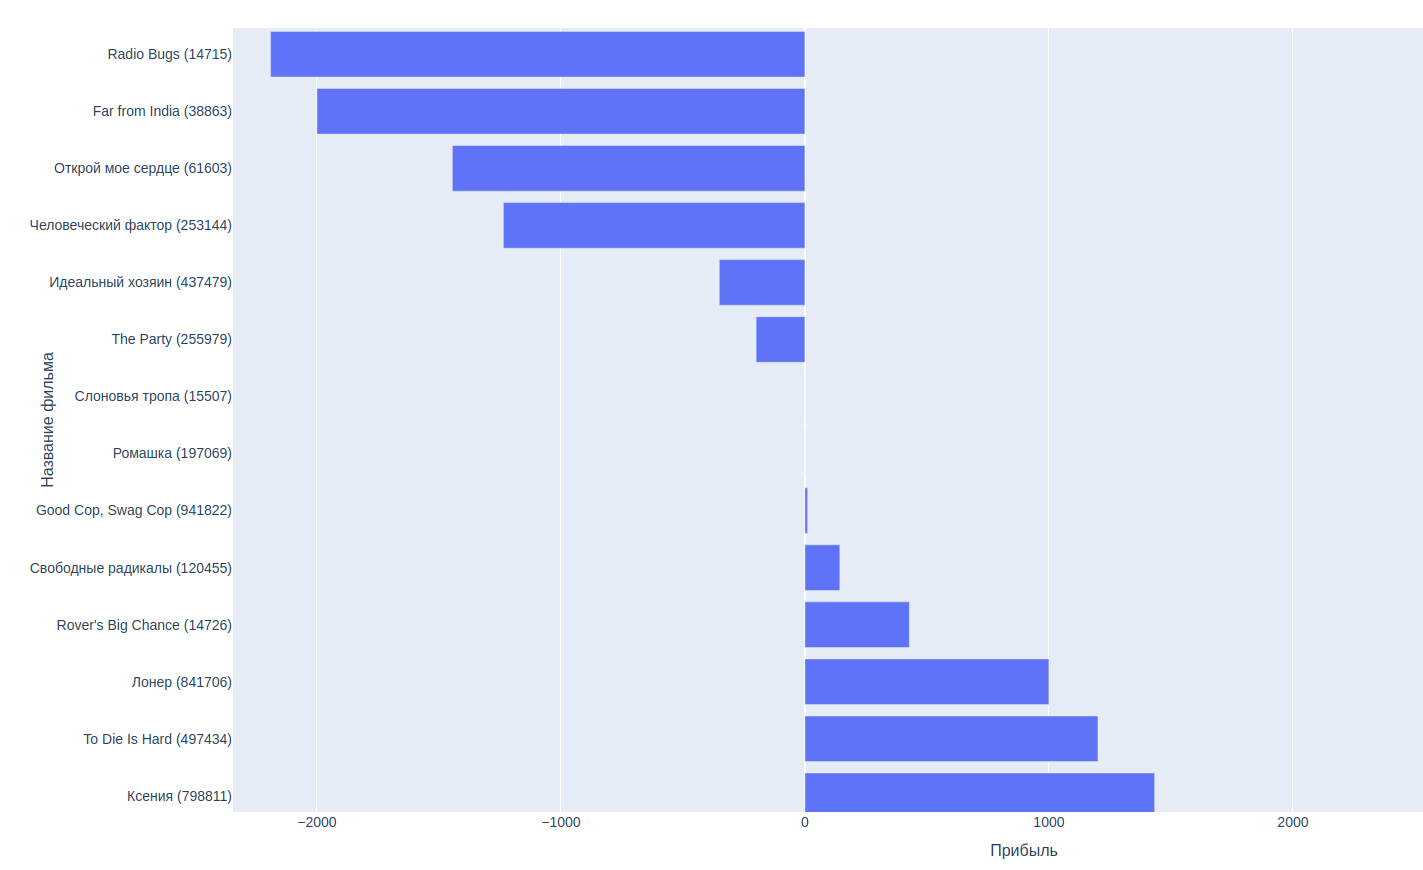
\includegraphics[width=\linewidth]{profit/zero}
			\caption{Фильмы с около нулевой прибылью}
			\label{fig:3}
		\end{figure}
	}
	\frame {
		\frametitle{Распределение фильмов по прибыльности (3)}
		\begin{figure}
			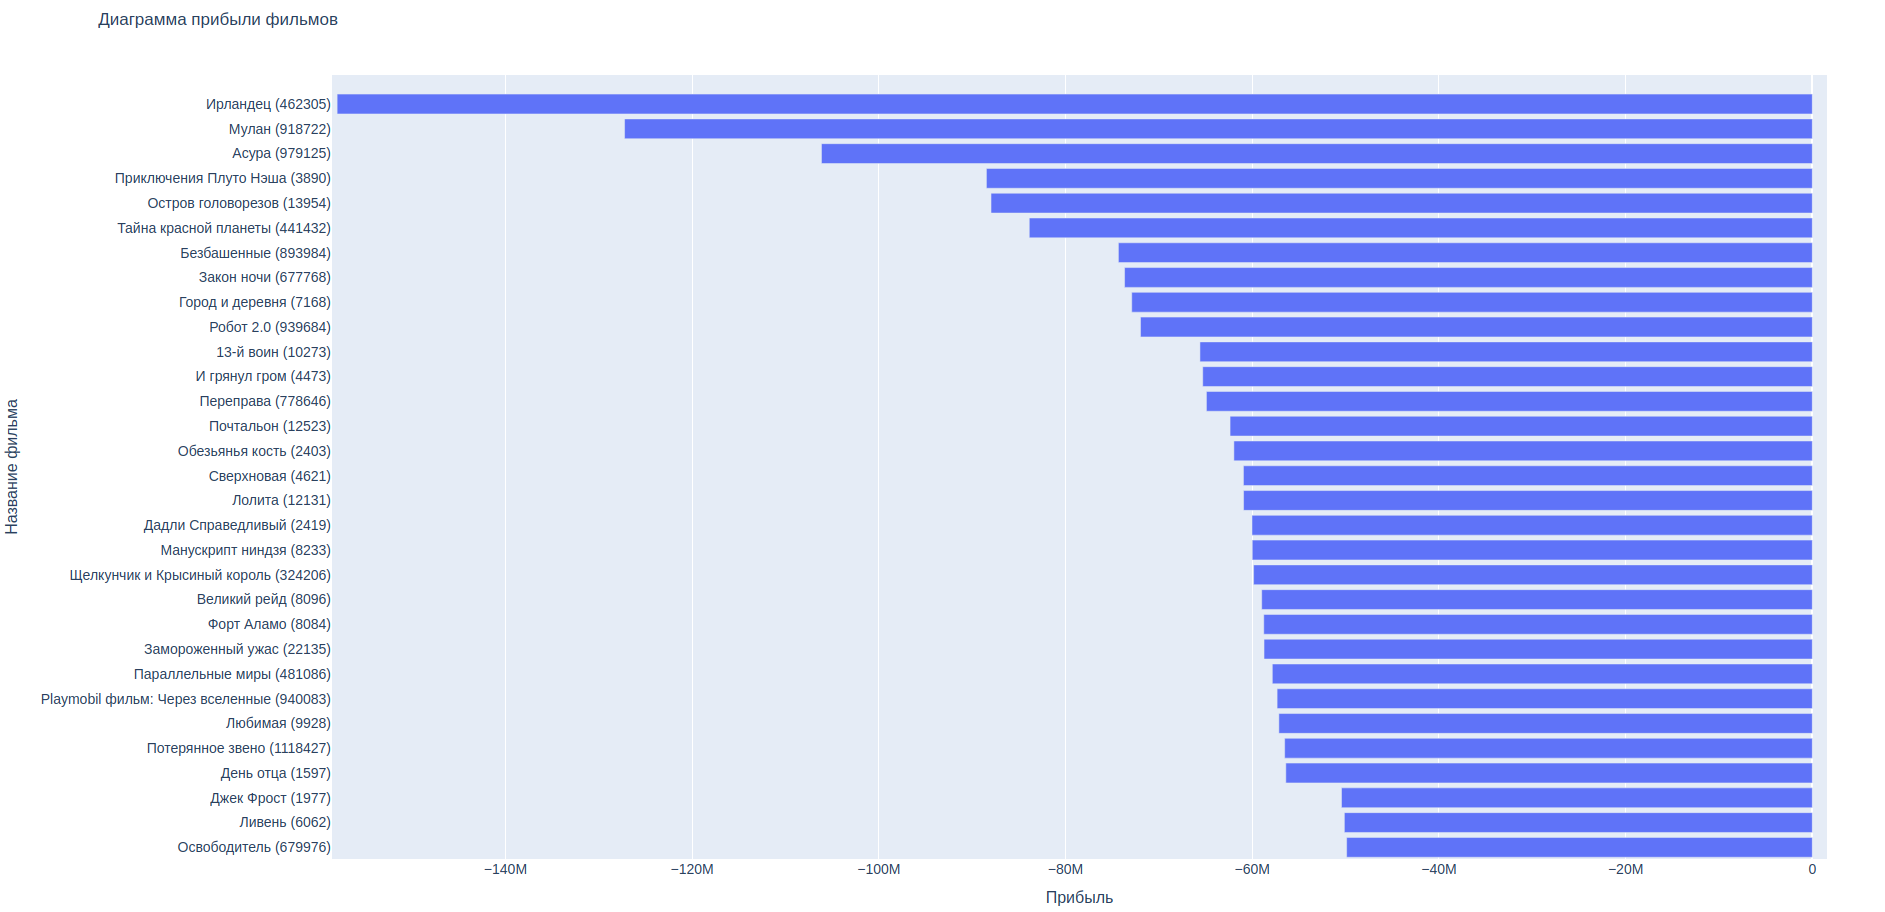
\includegraphics[width=\linewidth]{profit/worst}
			\caption{Самые неприбыльные фильмы}
			\label{fig:4}
		\end{figure}
	}
	\frame {
		\frametitle{Распределение фильмов по странам и годам}
	}
	\frame {
		\frametitle{Распределение фильмов по возрастным ограничениям и годам}
	}	
	\frame {
		\frametitle{Средний рейтинг российских фильмов по годам}
	}	

	\frame {
		\frametitle{Исследовательские задачи}
		
		\begin{itemize}
			\item Прогноз количества фильмов по жанрам на 10 лет
		\end{itemize}
	}
	\frame {
		\frametitle{Прогноз количества фильмов по жанрам на 10 лет}
	}	

\end{document}